\documentclass[notes,11pt, aspectratio=169]{beamer}
\usepackage[default]{lato}
%\usepackage{enumitem}
%\usepackage{color}
\newenvironment{transitionframe}{
  \setbeamercolor{background canvas}{bg=yellow}
  \begin{frame}}{
    \end{frame}
}


\setbeamercolor{frametitle}{fg=blue}
\setbeamercolor{title}{fg=black}
\setbeamertemplate{footline}[frame number]
\setbeamertemplate{navigation symbols}{} 
\setbeamertemplate{itemize items}{-}
\setbeamercolor{itemize item}{fg=blue}
\setbeamercolor{itemize subitem}{fg=blue}
\setbeamercolor{enumerate item}{fg=blue}
\setbeamercolor{enumerate subitem}{fg=blue}
\setbeamercolor{button}{bg=MyBackground,fg=blue,}
%\%setbeamercolor{block title}{fg=white,bg=blue}
%\setbeamercolor{block body}{fg=black,bg=gray}


% If you like road maps, rather than having clutter at the top, have a roadmap show up at the end of each section 
% (and after your introduction)
% Uncomment this is if you want the roadmap!
% \AtBeginSection[]
% {
%    \begin{frame}
%        \frametitle{Roadmap of Talk}
%        \tableofcontents[currentsection]
%    \end{frame}
% }
\setbeamercolor{section in toc}{fg=blue}
\setbeamercolor{subsection in toc}{fg=red}
\setbeamersize{text margin left=1em,text margin right=1em} 

\newenvironment{wideitemize}{\itemize\addtolength{\itemsep}{10pt}}{\enditemize}

%\documentclass[structure,compress,mathserif]{beamer}

\AtBeginSection[]{
  \begin{frame}
  \vfill
  \centering
  \begin{beamercolorbox}[sep=8pt,center,shadow=true,rounded=true]{title}
    \usebeamerfont{title}\insertsectionhead\par%
  \end{beamercolorbox}
  \vfill
  \end{frame}
}

\setbeamertemplate{caption}[numbered]
\usepackage{adjustbox}
\usepackage{threeparttable}
\usepackage{graphicx}
%\usepackage{chngcntr}
%\counterwithin{subfigure}{figure}
\usepackage{multicol}
\usepackage{natbib}
\usepackage{float}
\usepackage{url}
\usepackage{hyperref}
\usepackage{color}
\usepackage{tabls, calc}
\usepackage[tableposition=top]{caption}
\usepackage{ifthen}
\usepackage{setspace}
\usepackage{booktabs}
\usepackage[english]{babel}
\usepackage[latin1]{inputenc}
\usepackage{caption}
\usepackage{subfigure}	
%\usepackage{custom}
\usepackage{tikz}
\usepackage{array}
\usepackage{dcolumn}
\usepackage{multirow}
\usepackage{markdown}
\usepackage{siunitx}
\usepackage{tfrupee}
%\usepackage[table]{xcolor}
%\usepackage{xcolor}
\usepackage{colortbl}
\usepackage{tcolorbox}

\tcbset{width=0.9\textwidth,boxrule=0pt,colback=red,arc=0pt,auto outer arc,left=0pt,right=0pt,boxsep=5pt}


%%%%%%%%%%%%%%%%%%%%%%%%%%%%%5
\usepackage{listings}
\definecolor{codegreen}{rgb}{0,0.6,0}
\definecolor{codegray}{rgb}{0.5,0.5,0.5}
\definecolor{codepurple}{rgb}{0.58,0,0.82}
\definecolor{backcolour}{rgb}{0.95,0.95,0.92}

\lstdefinestyle{mystyle}{
    backgroundcolor=\color{backcolour},   
    commentstyle=\color{codegreen},
    keywordstyle=\color{magenta},
    numberstyle=\tiny\color{codegray},
    stringstyle=\color{codepurple},
    basicstyle=\ttfamily\footnotesize,
    breakatwhitespace=false,         
    breaklines=true,                 
    captionpos=b,                    
    keepspaces=true,                 
    numbers=left,                    
    numbersep=5pt,                  
    showspaces=false,                
    showstringspaces=false,
    showtabs=false,                  
    tabsize=2
}

\lstset{style=mystyle}


%%%%%%%%%%%%%%%%%%%%%%%%%%%%
\newcommand{\Note}[1]{
\rule{2.5cm}{0.25pt} \\ \textit{\footnotesize{\textcolor{rubineRed}{Note:} \textcolor{darkerGray}{#1}}}}

\newcommand{\formula}[1]{
\begin{beamerboxesrounded}[shadow = false, lower = formula body]{}
#1
\end{beamerboxesrounded}
}

\setbeamercolor{prac ques body}{fg=oiB}

\newcommand{\pq}[1]{
\begin{beamerboxesrounded}[shadow = false, lower = prac ques body]{}
#1
\end{beamerboxesrounded}
}



%%%%%%%%%%%%%%%%%%%%%%%%%%%%%%%
\newcommand{\hl}[1]{\textit{\textcolor{hlblue}{#1}}}
\newcommand{\hlGr}[1]{\textit{\textcolor{lightGreen}{#1}}}
\newcommand{\mathhl}[1]{\textcolor{hlblue}{\ensuremath{#1}}}


%%%Define Colors Here
\definecolor{applegreen}{rgb}{0.55, 0.71, 0.0}
\definecolor{ao(english)}{rgb}{0.0, 0.5, 0.0}
\definecolor{pink}{rgb}{0.858, 0.188, 0.478}
\definecolor{purple}{rgb}{0.59, 0.44, 0.84}
\definecolor{denim}{rgb}{0.08, 0.38, 0.74}
\definecolor{seagreen}{rgb}{0.13, 0.7, 0.67}
\definecolor{tangerine}{rgb}{0.95, 0.52, 0.0}
\definecolor{textboxgreen}{rgb}{0.67, 0.88, 0.69}
\definecolor{textboxred}{HTML}{BF616A}
\definecolor{backcolour}{rgb}{0.95,0.95,0.92}
\xdefinecolor{oiB}{rgb}{0.22,0.52,0.72}
\definecolor{oiG}{rgb}{.298,.447,.114}
\xdefinecolor{hlblue}{rgb}{0.051,0.65,1}
\xdefinecolor{gray}{rgb}{0.5, 0.5, 0.5}
\xdefinecolor{darkGray}{rgb}{0.3, 0.3, 0.3}
\xdefinecolor{darkerGray}{rgb}{0.2, 0.2, 0.2}
\xdefinecolor{rubineRed}{rgb}{0.89,0,0.30}
\xdefinecolor{irishGreen}{rgb}{0,0.60,0}	
\definecolor{lightGreen}{rgb}{0.387,0.581,0.148} 
\setbeamercolor{frametitle}{fg=denim}


%$%%%%%%%%%%%%%%%%%%%%%%%%%%%%%%%%%
\newcommand{\dq}[1]{
\begin{beamerboxesrounded}[shadow = false, lower = disc ques body]{}
#1
\end{beamerboxesrounded}
}

% solnMult: solutions for practice questions

\newcommand{\solnMult}[1]{
\item[] \vspace{-0.59cm}
\only<1>{\item #1}
\soln{\only<2->{\item \orange{#1}}}
}



%%%%%%%%%%%%%%%%%%%%%%%%%%%%%%%%%%%%%

%----------------------------------------------------------------------------------------
%	TITLE PAGE
%----------------------------------------------------------------------------------------
\title[DAR]{Data Analytics with R}  % The short title appears at the bottom of 
\author{Sumit Mishra} % Your name
\institute[IFMR] % Your institution as it will appear on the bottom of every slide, may be shorthand to save space
{
Institute for Financial Management and Research, Sri City \\ % Your institution for the title page
\medskip
\medskip
\textbf{Summarizing Data} % Your email address
}
\date{04 November 2020} % Date, can be changed to a custom date

%Preamble for ESTOUT
% *****************************************************************
% Estout related things
% *****************************************************************
\newcommand{\sym}[1]{\rlap{#1}}% Thanks to David Carlisle

\let\estinput=\input% define a new input command so that we can still flatten the document

\newcommand{\estwide}[3]{
		\vspace{.75ex}{
			\begin{tabular*}
			{\textwidth}{@{\hskip\tabcolsep\extracolsep\fill}l*{#2}{#3}}
			\toprule
			\estinput{#1}
			\bottomrule
			\addlinespace[.75ex]
			\end{tabular*}
			}
		}	

\newcommand{\estauto}[3]{
		\vspace{.75ex}{
			\begin{tabular}{l*{#2}{#3}}
			\toprule
			\estinput{#1}
			\bottomrule
			\addlinespace[.75ex]
			\end{tabular}
			}
		}

% Allow line breaks with \\ in specialcells
	\newcommand{\specialcell}[2][c]{%
	\begin{tabular}[#1]{@{}c@{}}#2\end{tabular}}

% *****************************************************************
% Custom subcaptions
% *****************************************************************
% Note/Source/Text after Tables
\newcommand{\figtext}[1]{
	\vspace{-1.9ex}
	\captionsetup{justification=justified,font=footnotesize}
	\caption*{\hspace{6pt}\hangindent=1.5em #1}
	}
\newcommand{\fignote}[1]{\figtext{\emph{Note:~}~#1}}

\newcommand{\figsource}[1]{\figtext{\emph{Source:~}~#1}}

% Add significance note with \starnote
\newcommand{\starnote}{\figtext{* p < 0.1, ** p < 0.05, *** p < 0.01. Standard errors in parentheses.}}

% *****************************************************************
% siunitx
% *****************************************************************
\usepackage{siunitx} % centering in tables
	\sisetup{
		detect-mode,
		tight-spacing		= true,
		group-digits		= false ,
		input-signs		= ,
		input-symbols		= ( ) [ ] - + *,
		input-open-uncertainty	= ,
		input-close-uncertainty	= ,
		table-align-text-post	= false
        }
%Preamble ends here 
%%%%%%%%%%%%%%%%%%%%%%%%%%%%%%%%%%%%%%%%%%%%%%%%%%%%%%%%%%%%%%%%%%%%%%%%%
%%%%%%%%%%%%%%%%%%%%%%%%%%%%%%%%%%%%%%%%%%%%%%%%%%%%%%%%%%%%%%%%%%%%%%%%%
              
\begin{document}
\begin{frame}
  \titlepage
\end{frame}

\begin{frame}{Agenda}
\begin{itemize}
\item Examining numerical data
\item Examining categorical data
\item Case study: Racial discrimination in job-market.
\item Material: Textbook chapter 02.
\end{itemize}
\end{frame}


\section{Examining Numerical Data}
\begin{frame}{Scatterplot for paired data}
\textcolor{purple}{Scatterplots} are useful for visualizing the relationship between two numerical variables.
\begin{center}
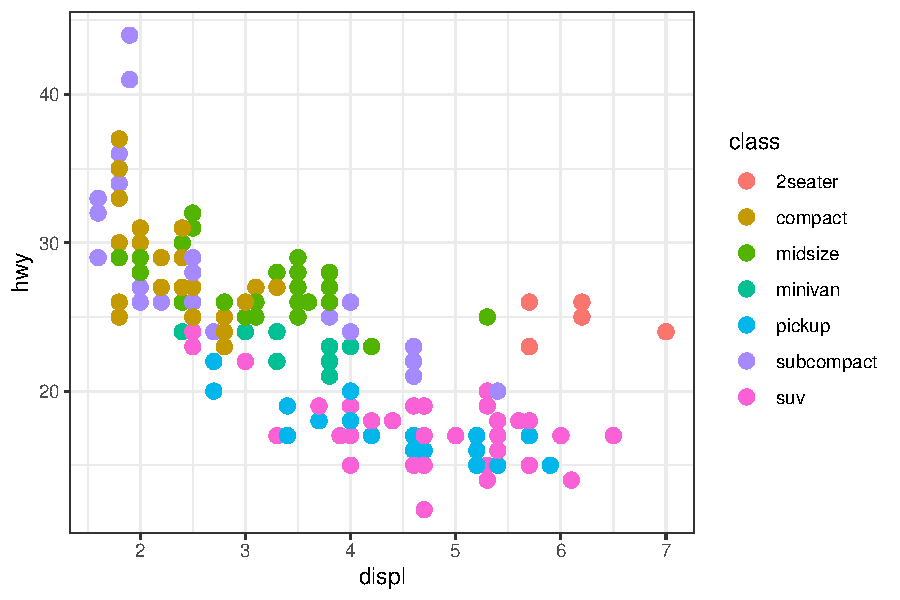
\includegraphics[width=0.7\textwidth]{graphs/l02f01.pdf}
\end{center}
\end{frame}


\begin{frame}{Dot plot}
These are useful to visualize one numerical variable. Darker colors represent greater concentration of observations.
\begin{center}
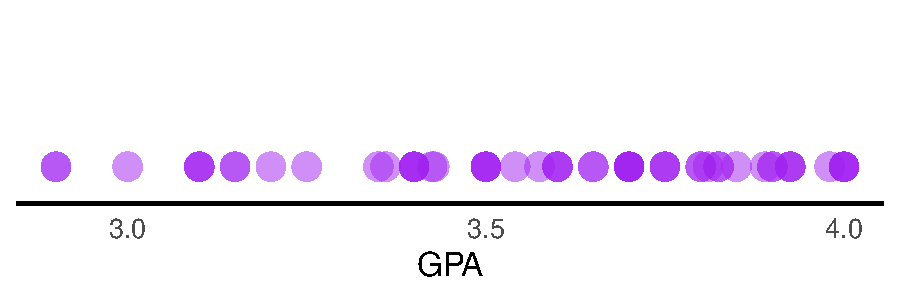
\includegraphics[width=0.5\textwidth]{graphs/l02f02.pdf}
\end{center}
\end{frame}

\begin{frame}{Dot plot with mean}
\begin{center}
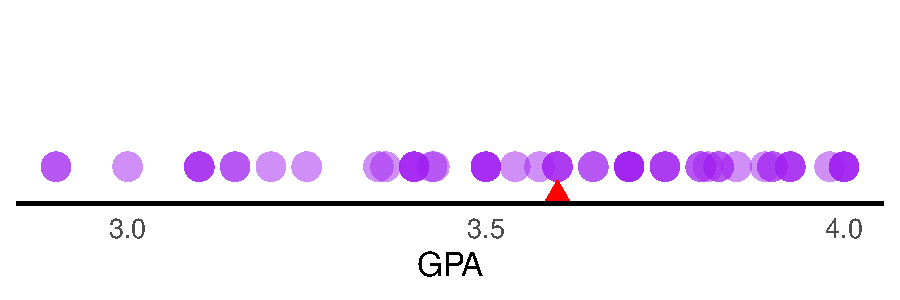
\includegraphics[width=0.5\textwidth]{graphs/l02f03.pdf}
\end{center}
\pause

\begin{itemize}
\item The \textcolor{red}{mean} represents the center of the distribution.
\item The \textcolor{red}{mean} GPA is \pause \textcolor{purple}{3.59}.
\end{itemize}
\end{frame}


\begin{frame}[fragile]{Exercise}
\begin{center}
Construct dot plot for the variable \texttt{interest\_rate} from the dataset \texttt{loan50}.
\end{center}

\pause

\begin{columns}
 \column{.6\linewidth}
      \centering
\begin{lstlisting}[language=R]
  loan50 %>% 
  ggplot(aes(x =interest_rate)) + 
  geom_dotplot(fill = "steelblue", color = "steelblue",
               alpha = 0.8, binwidth = 0.9) + 
  guides(y = "none") + 
  labs(y = NULL, x = "Interest Rate") + 
  scale_x_continuous(breaks = c(5, 10, 15, 20, 25)) + 
  theme_minimal() + 
  geom_point(aes(x = mean(interest_rate), y=0), 
             shape = 17, size = 6, color = "red") +
  theme(axis.line.x = element_line(),
        panel.grid = element_blank())

\end{lstlisting}

\pause

\column{.38\linewidth}
      \centering
      \begin{figure}
      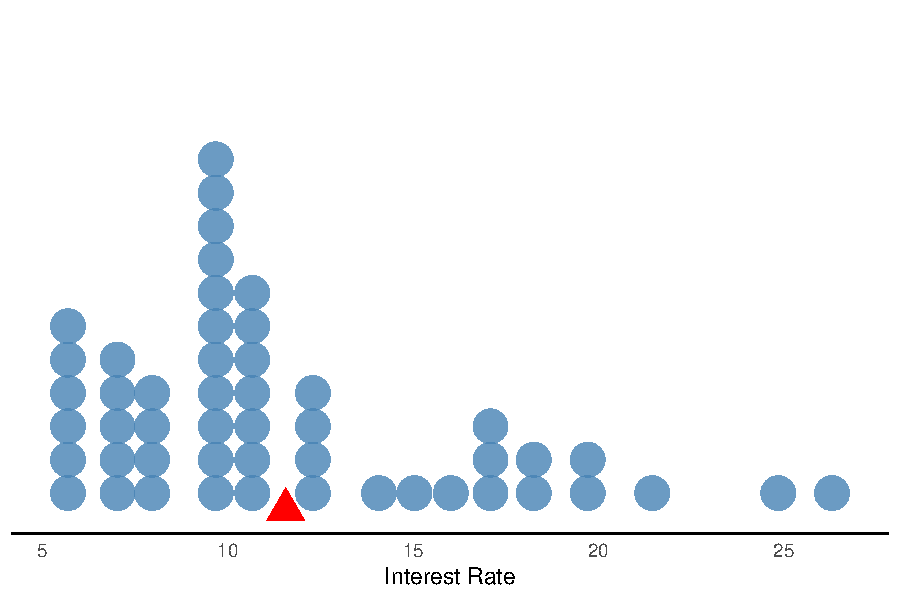
\includegraphics[scale=0.5]{graphs/l02f04.pdf}
      \end{figure}
\end{columns}
\end{frame}


\begin{frame}{Mean}

\begin{center}
\colorbox{textboxgreen}{
 The sample mean, denoted as $\bar{x}$ , can be calculated as 
$\bar{x}  = \frac{x_1 + x_2 + .... + x_n}{n}$ }

\vspace{4mm}

\colorbox{textboxred}{
The population mean, denoted by $\mu$, is an elusive quantity.
}

\vspace{4mm}

\colorbox{textboxgreen!65}{
We assume that $\bar{x}$ (an estimate of the population mean) is a good way to represent $\mu$.
}
\end{center}
\end{frame}


\begin{frame}[fragile]{Histogram}
\begin{figure}[ht]
\centering\small
\begin{tabular}{l ccc ccc ccc}
  \hline
  Interest Rate &
      5.0\% - 7.5\% &
      7.5\% - 10.0\% &
      10.0\% - 12.5\% &
      12.5\% - 15.0\% &
      $\cdots$ &
      25.0\% - 27.5\% \\
  \hline
  Count & 11 & 15 & 8 & 4 & $\cdots$ & 1 \\
  \hline
\end{tabular}
\caption{Counts for the binned
    \texttt{interest\_rate} data.}
\label{binnedIntRateAmountTable}
\end{figure}

\pause

\begin{columns}
 \column{.5\linewidth}
      \centering
   \begin{lstlisting}[language=R]
   hist(loan50$interest_rate,
          col = "steelblue", main = NULL,
           xlab = "Interest Rate", ylab = NULL) 
   \end{lstlisting}
\pause

\column{.44\linewidth}
      \centering
      \begin{figure}
      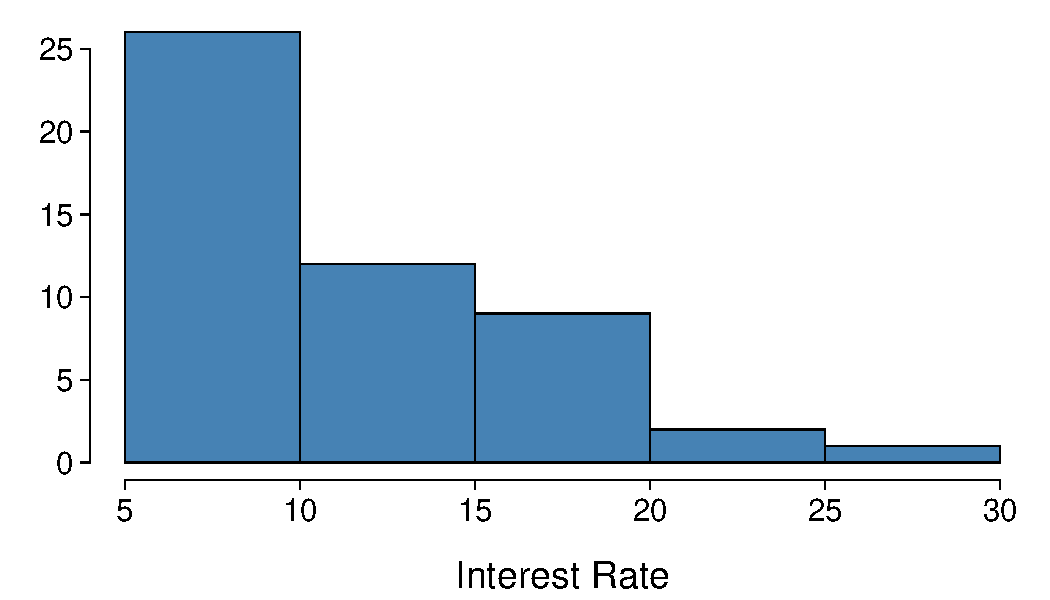
\includegraphics[scale=0.4]{graphs/l02f05.pdf}
      \end{figure}
\end{columns}
\end{frame}

\begin{frame}{Shape of a distribution: Modality}
Does the histogram have a single prominent peak (\hl{unimodal}), several prominent peaks (\hl{bimodal/multimodal}), or no apparent peaks (\hl{uniform})?

\begin{center}
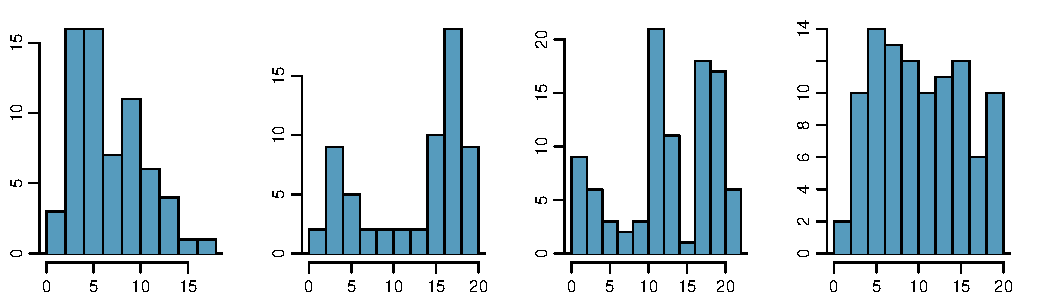
\includegraphics[width=0.75\textwidth]{graphs/l02f06}
\end{center}

\Note{In order to determine modality, step back and imagine a smooth curve over the histogram -- imagine that the bars are wooden blocks and you drop a limp spaghetti over them, the shape the spaghetti would take could be viewed as a smooth curve.}
\end{frame}


\begin{frame}
\frametitle{Shape of a distribution: skewness}

Is the histogram \hl{right skewed}, \hl{left skewed}, or \hl{symmetric}?

\begin{center}
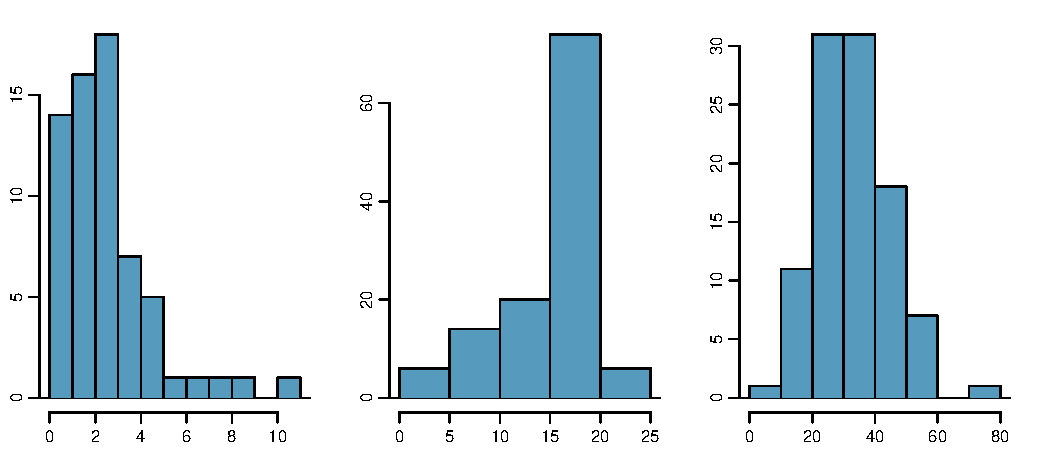
\includegraphics[width=0.8\textwidth]{graphs/l02f07.pdf}
\end{center}

\Note{Histograms are said to be skewed to the side of the long tail.}

\end{frame}


\begin{frame}
\frametitle{Shape of a distribution: unusual observations}

Are there any unusual observations or potential \hl{outliers}?

\begin{center}
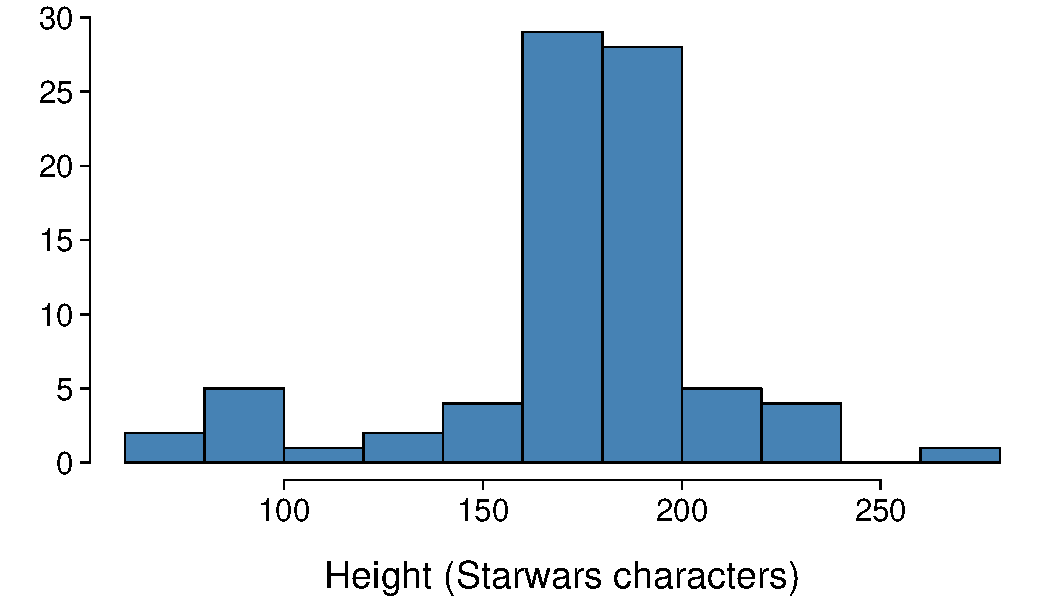
\includegraphics[width=0.65\textwidth]{graphs/l02f08.pdf}
\end{center}

\pause 

Plot the variable \texttt{mass} from \texttt{starwars} dataset, and look for outliers.
\end{frame}


\begin{frame}{Extracurricular activities}

\dq{How would you describe the shape of the distribution of hours per week students spend on extracurricular activities?}

\begin{center}
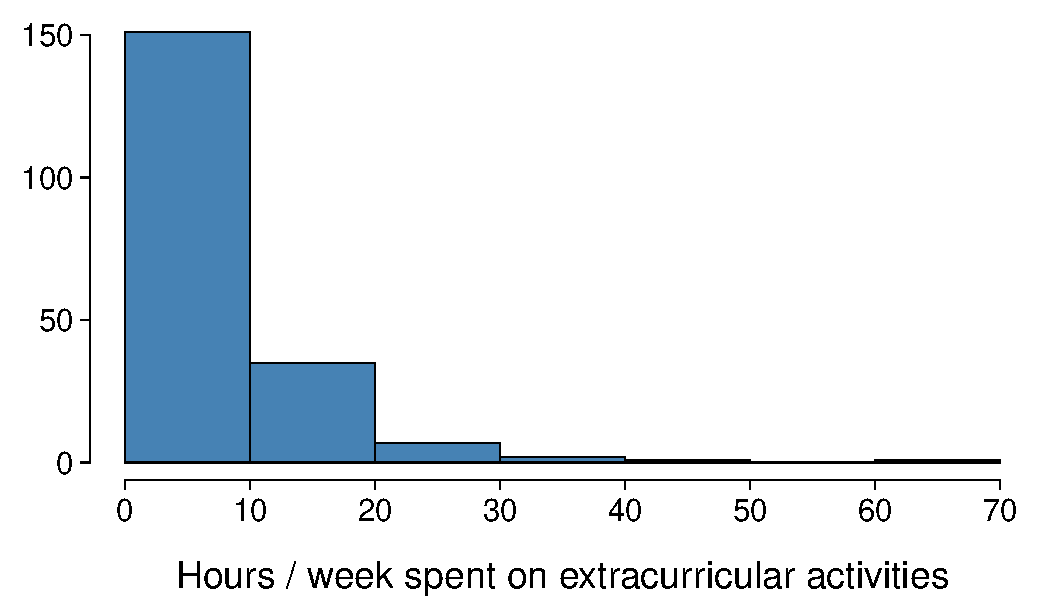
\includegraphics[width=0.55\textwidth]{graphs/l02f09.pdf}
\end{center}

\pause
\colorbox{textboxgreen!75}{\textit{Unimodal and right skewed, with an outlier at 60 hours/week.}}

\end{frame}


\begin{frame}
\frametitle{Commonly observed shapes of distributions}

\begin{itemize}

\item modality \\
$\:$ \\
\pause

\begin{columns}[c]
\column{0.25\textwidth}
unimodal \\
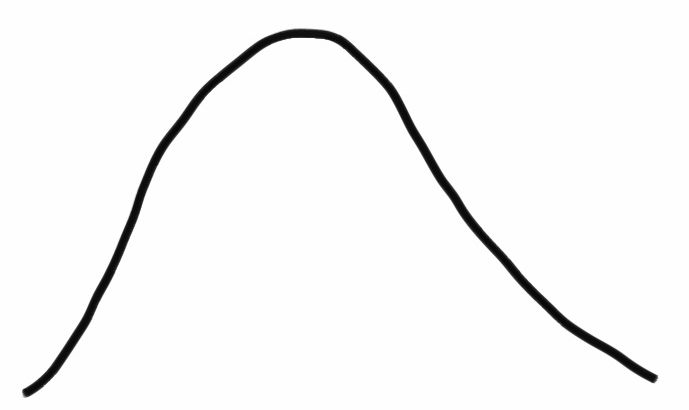
\includegraphics[width=\textwidth]{graphs/shape_sketches/unimodal} 
\pause
\column{0.25\textwidth}
bimodal \\
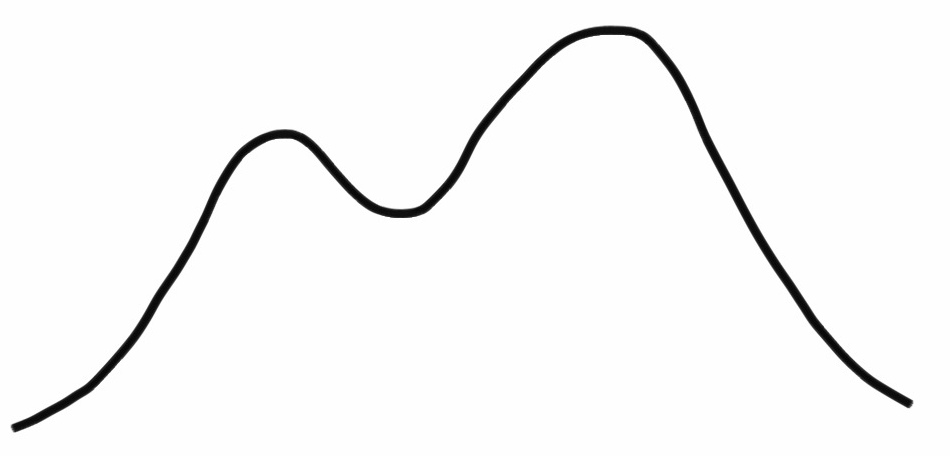
\includegraphics[width=\textwidth]{graphs/shape_sketches/bimodal} 
\pause
\column{0.25\textwidth}
multimodal \\
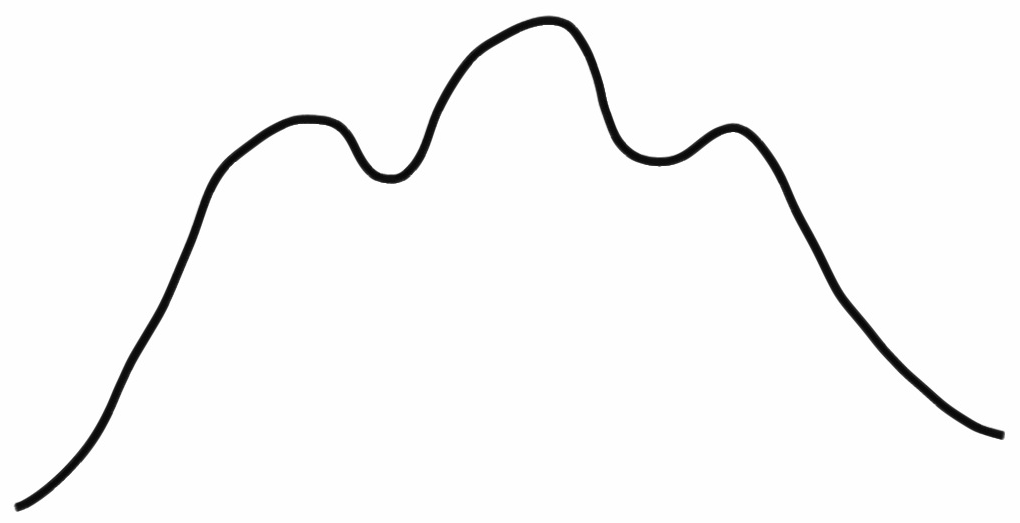
\includegraphics[width=\textwidth]{graphs/shape_sketches/multimodal} 
\pause
\column{0.25\textwidth}
uniform
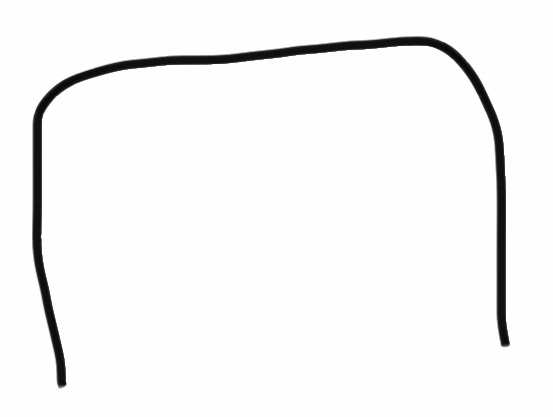
\includegraphics[width=\textwidth]{graphs/shape_sketches/uniform} 
\end{columns}

\pause

$\:$ \\

\item skewness \\
$\:$ \\
\pause

\begin{columns}[c]
\column{0.25\textwidth}
right skew \\
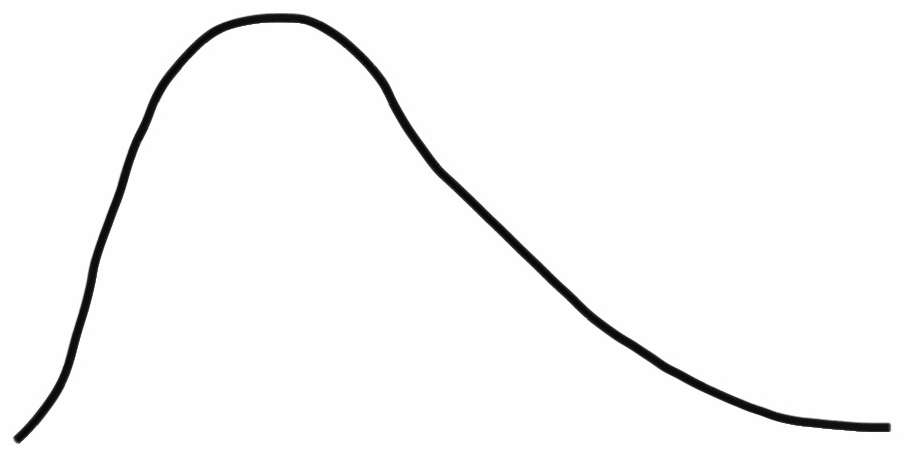
\includegraphics[width=\textwidth]{graphs/shape_sketches/right_skew} 
\pause
\column{0.25\textwidth}
left skew \\
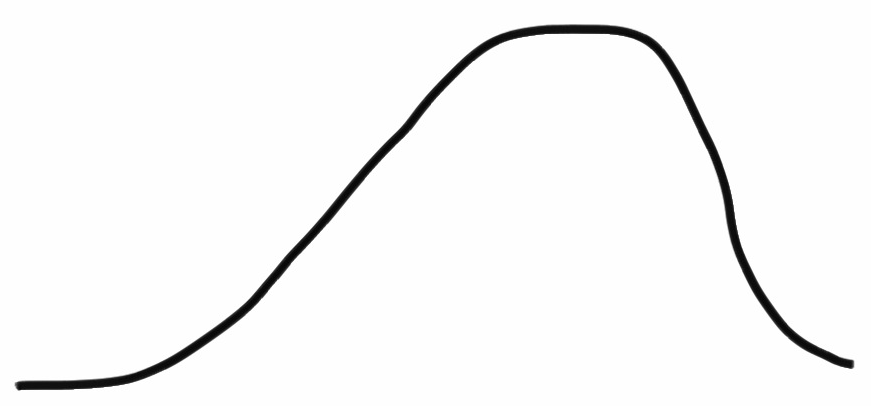
\includegraphics[width=\textwidth]{graphs/shape_sketches/left_skew} 
\pause
\column{0.25\textwidth}
symmetric \\
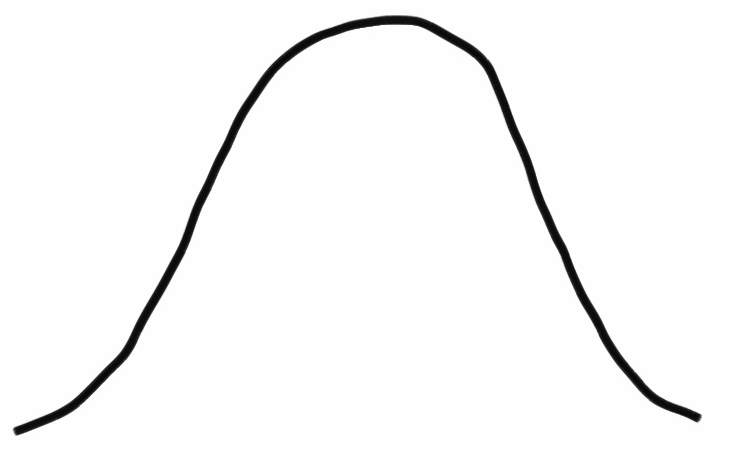
\includegraphics[width=\textwidth]{graphs/shape_sketches/symmetric} 
\end{columns}

\end{itemize}

\end{frame}


\begin{frame}{Variance}
\begin{center}
\colorbox{textboxgreen}{
 The variance, denoted as $V(x)$ , can be calculated as 
$ V(x) = \frac{\sum_{i = 1}^n (x_i - \bar{x})^2}{n - 1}$  }

\vspace{5mm}

\pause

\colorbox{textboxred!75}{\parbox{0.75\textwidth}{
Compute the variance for the variable \texttt{height} from the dataset \texttt{starwars} with
 and without using the canned function.}}
\end{center}


\pause
\vspace{8mm}

\begin{wideitemize}
\item We square up the deviations so that only the distance (and not the direction) matters.
\item Larger deviations (irrespective of the direction) get greater weightage. 
\end{wideitemize}
\end{frame}

\begin{frame}{Standard Deviation}

\begin{center}
\colorbox{textboxgreen}{\parbox{0.85\textwidth}{
The standard deviation is the square root of the variance $V(x)$, and has the same units as the data

 \vspace{1mm}
 
 $ s = \sqrt{V(x)}$ }}
\end{center}

\end{frame}


\begin{frame}{Median}

\begin{itemize}

\item The \hl{median} is the value that splits the data in half when ordered in ascending order.

\[ 0,1,\textcolor{tangerine}{2},3,4 \]

\item If there are an even number of observations, then the median is the average of the two values in the middle.

\[ 0,1,\underline{2,3},4,5 \rightarrow \frac{2 + 3}{2} = \textcolor{tangerine}{2.5} \]

\item Since the median is the midpoint of the data, 50\% of the values are below it. Hence, it is also the \hl{$50^{th}$ percentile}.

\end{itemize}

\end{frame}

\begin{frame}[fragile]{Q1, Q3, and IQR}

\begin{itemize}

\item The $25^{th}$ percentile is also called the first quartile, \hl{Q1}.

\item The $50^{th}$ percentile is also called the median.

\item The $75^{th}$ percentile is also called the third quartile, \hl{Q3}.

\item Between Q1 and Q3 is the middle 50\% of the data. The range these data span is called the \hl{interquartile range}, or the \hl{IQR}.
\formula{\[ IQR = Q3 - Q1 \]}
\end{itemize}

\end{frame}

\begin{frame}{Boxplot}
The box in a \hl{box plot} represents the middle 50\% of the data, and the thick line in the box is the median.

\begin{center}
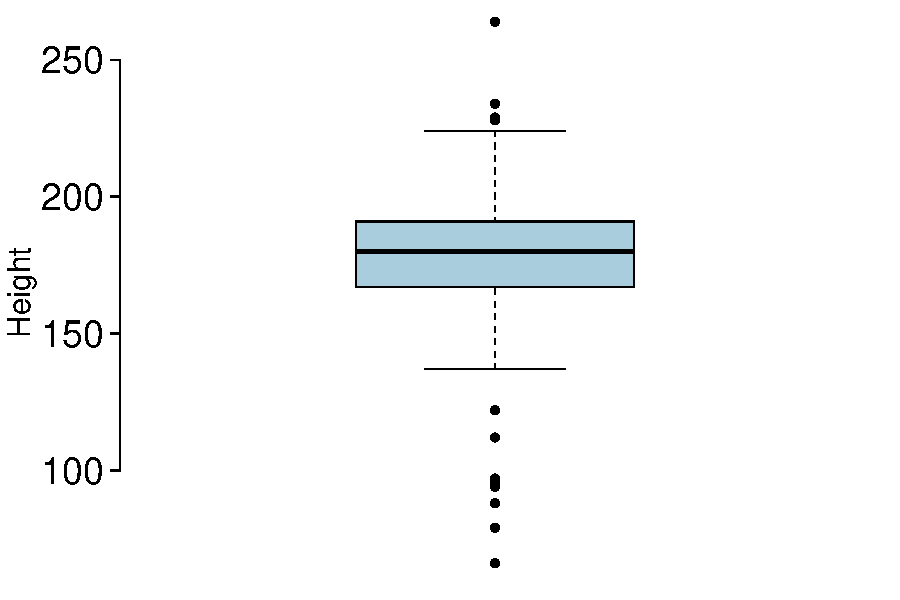
\includegraphics[width=0.7\textwidth]{graphs/l02f10.pdf}
\end{center}

\end{frame}


\begin{frame}{Boxplot Explained}

\begin{center}
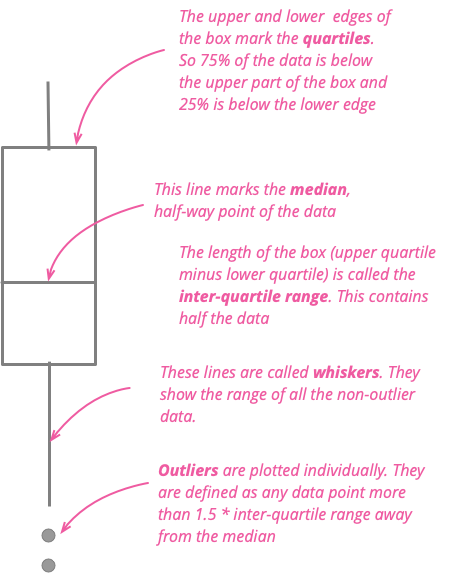
\includegraphics[width=0.3\textwidth]{graphs/boxplotExplainer.png}
\end{center}


 \Note{As an aside, this is a nice blog post on comparing groups (I have added the nice boxplot explainer from this piece) that you should read- \url{https:
//martinfowler.com/articles/dont-compare-averages.html}}
\end{frame}

\begin{frame}[fragile]{Whiskers and outliers}
\begin{itemize}
\item \hl{Whiskers} of a box plot can extend up to $1.5 \times IQR$ away from the quartiles.
\formula{
\vspace{-0.5cm}
\begin{align*} 
\text{max~upper~whisker~reach} &= Q3 + 1.5 \times IQR \\
\text{max~lower~whisker~reach} &= Q1 - 1.5 \times IQR
\end{align*}
}
\pause
\vspace{-0.5cm}
{\small
\begin{align*}
\text{IQR}&: 191 - 167 = 24 \\
\text{max~upper~whisker~reach}&= 191 + 1.5\times 24 = 227 \\
\text{max~lower~whisker~reach}&= 167 - 1.5\times 24 = 131
\end{align*}
}

\pause
\vspace{-0.25cm}
\item A potential \hl{outlier} is defined as an observation beyond the maximum reach of the whiskers. It is an observation that appears extreme relative to the rest of the data.
\end{itemize}
\end{frame}


%%%%%%%%%%%%%%%%%%%%%%%%%%%%%%%
\begin{frame}[fragile]{Mean vs. median}

\begin{itemize}

\item If the distribution is symmetric, center is often defined as the mean: mean $\approx$ median

\begin{center}
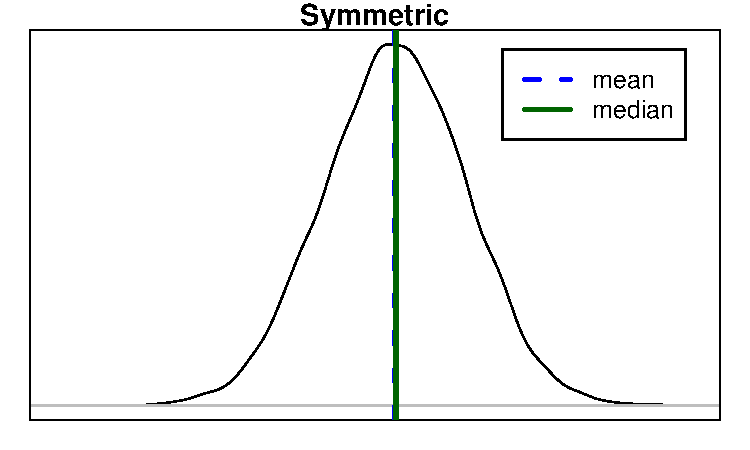
\includegraphics[width=0.33\textwidth]{graphs/l02f11/sym}
\end{center}

\item If the distribution is skewed or has extreme outliers, center is often defined as the median
\begin{itemize}
\item Right-skewed: mean $>$ median
\item Left-skewed: mean $<$ median \\
\end{itemize}

\end{itemize}

\begin{center}
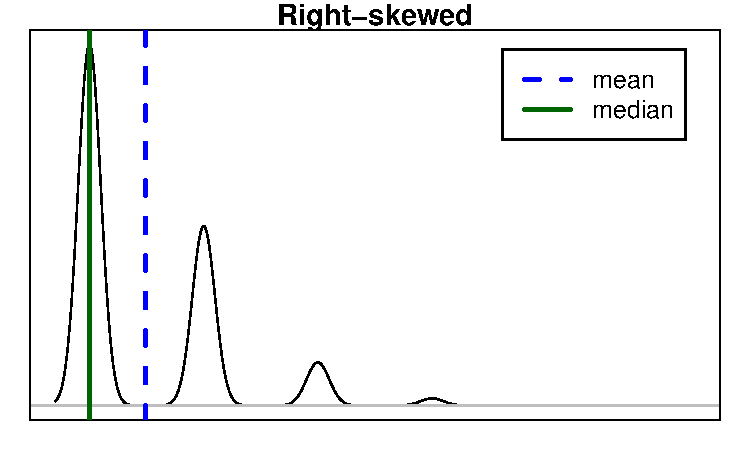
\includegraphics[width=0.3\textwidth]{graphs/l02f11/rs}
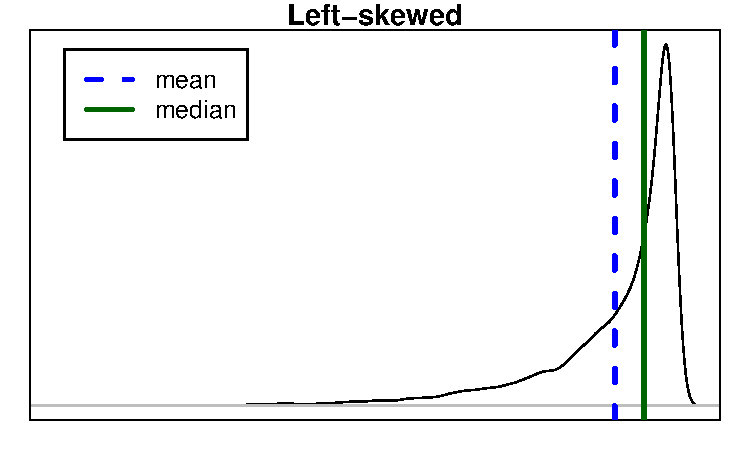
\includegraphics[width=0.3\textwidth]{graphs/l02f11/ls}\\
\end{center}

\end{frame}


%%%%%%%%%%%%%%%%%%%%%%%%%%%%%%%

\begin{frame}
\frametitle{Practice}

\pq{{\small Which is most likely true for the distribution of percentage of time actually spent taking notes in class versus on Facebook, Twitter, etc.?}}

\vspace{-0.5cm}

\begin{columns}
\column{0.7\textwidth}
\begin{center}
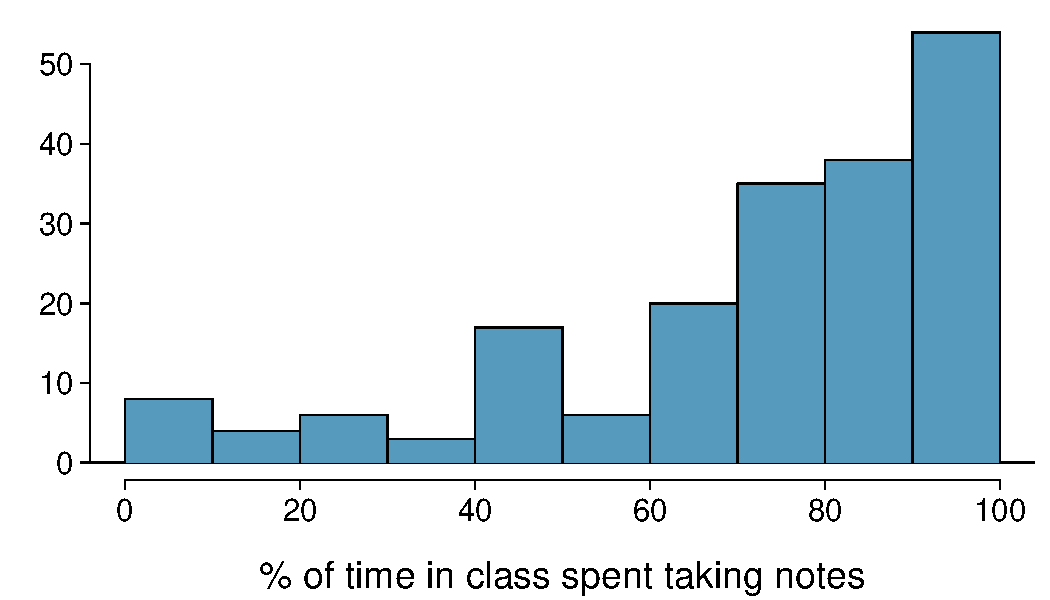
\includegraphics[width=0.6\textwidth]{graphs/l02f12.pdf}
\end{center}
\end{columns}

{\small
\begin{enumerate}[(a)]
\item mean$>$ median
\item mean $<$ median
\item mean $\approx$ median
\item impossible to tell
\end{enumerate}
}

\end{frame}


%%%%%%%%%%%%%%%%%%%%%%%%%%%%%%%

\begin{frame}
\frametitle{Practice}

\pq{{\small Which is most likely true for the distribution of percentage of time actually spent taking notes in class versus on Facebook, Twitter, etc.?}}

\vspace{-0.5cm}

\begin{columns}
\column{0.7\textwidth}
\begin{center}
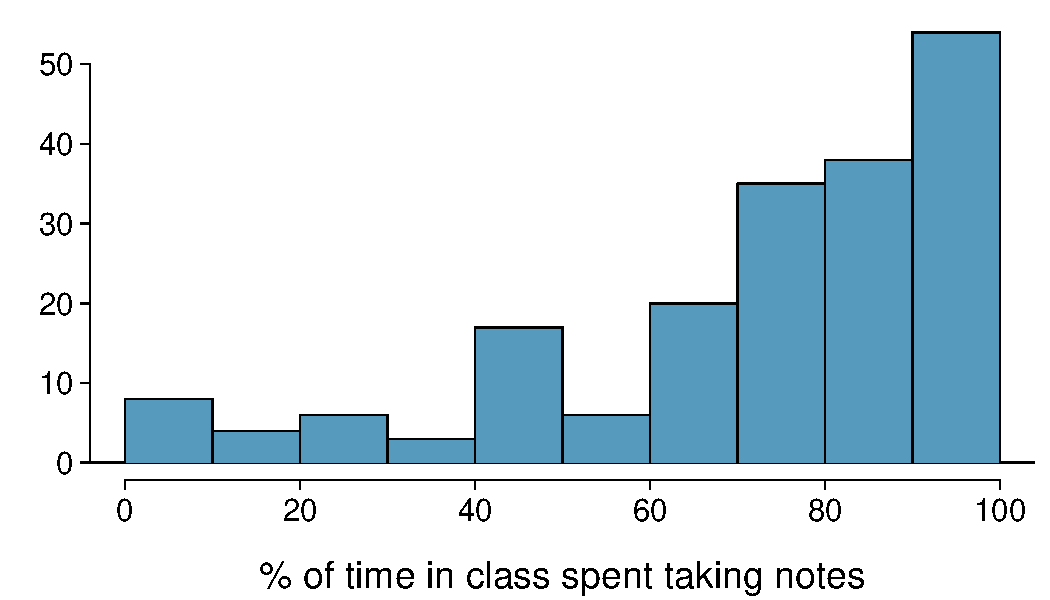
\includegraphics[width=0.6\textwidth]{graphs/l02f12.pdf}
\end{center}
\column{0.3\textwidth}
$\:$ \\
$\:$ \\
\textcolor{orange}{median: 80\% \\ mean: 76\%}
\end{columns}

{\small
\begin{enumerate}[(a)]
\item mean$>$ median
\item \textcolor{orange}{mean $<$ median}
\item mean $\approx$ median
\item impossible to tell
\end{enumerate}
}

\end{frame}



%%%%%%%%%%%%%%%%%%%%%%%%%%%%%%%
\begin{frame}[fragile]{Extremely Skewed Distribution}

When data are extremely skewed, transforming them might make modeling easier. A common transformation is the \hl{log transformation}.

$\:$ \\
\pause
The histogram on the left shows the distribution of mass of Star Wars characters. The histogram on the right shows the distribution of log of mass.

\begin{columns}
\column{.48\linewidth}
\begin{center}
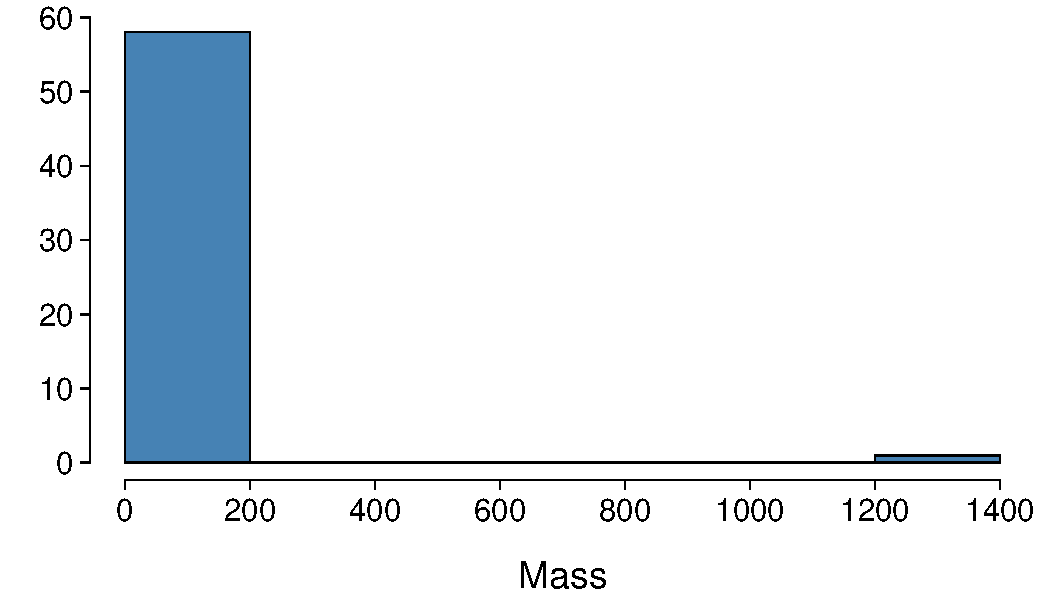
\includegraphics[scale=0.4]{graphs/l02f13a.pdf}
\captionof{figure}{How it started}
\end{center}

\column{.48\linewidth}
\begin{center}
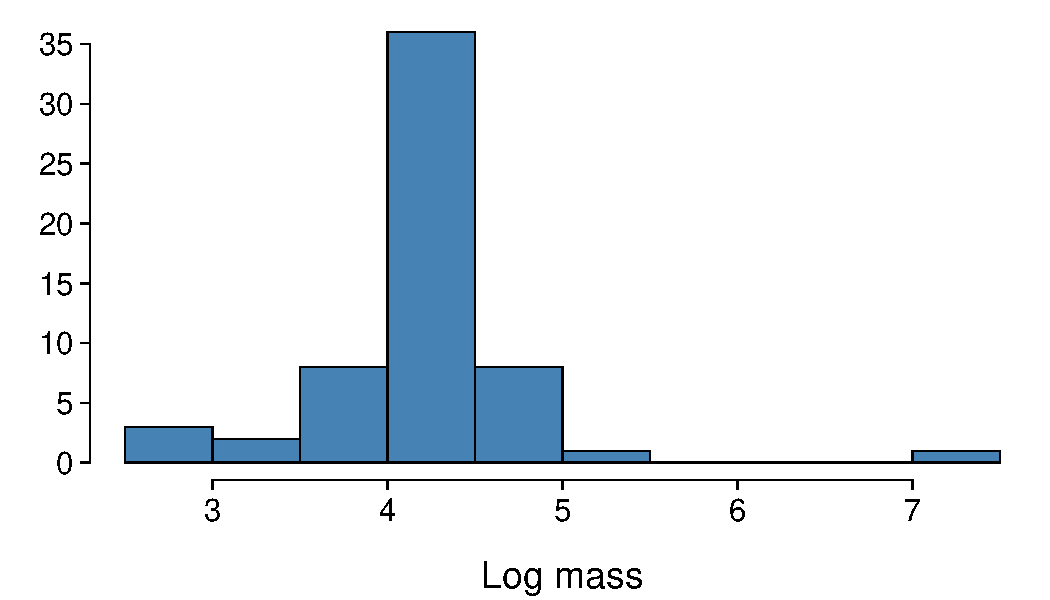
\includegraphics[scale=0.4]{graphs/l02f13b.pdf}
\captionof{figure}{How it's going}
\end{center}
\end{columns}
\end{frame}


%%%%%%%%%%%%%%%%%%%%%%%%%%%%%%%
%%%%%%%%%%%%%%%%%%%%%%%%%%%%%%%

\section{Considering Categorical Data}

%%%%%%%%%%%%%%%%%%%%%%%%%%%%%%%

\begin{frame}{Contingency Table}
A table that summarizes data for two categorical variables is called a \hl{contingency table}.

$\:$ \\
\pause
The contingency table below shows the distribution of callback rate and race of applicants.

\begin{center}
\begin{tabular}{l l cc r}
					               & 			 & \multicolumn{2}{c}{{Callback}} \\
  \cline{3-4}
					               &			 & No	 & Yes	& Total \\ 
  \cline{2-5}
\multirow{2}{*}{{Race}}& Black & 2278  & 157	  	& 2435 \\ 
  					             & White & 2200	 & 235 	    & 2435 \\ 
  \cline{2-5}
  					             & Total & 4478  & 392	    &  4870 \\
  \cline{2-5}
\end{tabular}
\end{center}
\end{frame}


%%%%%%%%%%%%%%%%%%%%%%%%%%%%%%%%%%

\begin{frame}[fragile]{Bar plots}

A \hl{bar plot} is a common way to display a single categorical variable. A bar plot where proportions instead of frequencies are shown is called a \hl{relative frequency bar plot}.

\begin{center}
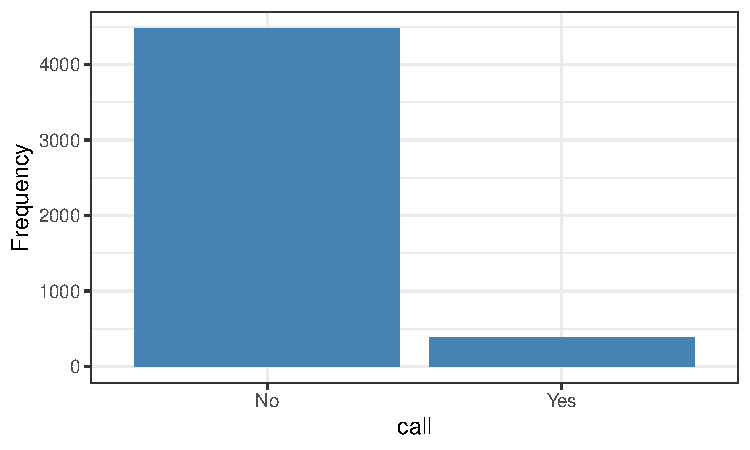
\includegraphics[width=0.45\textwidth]{graphs/l02f14a}
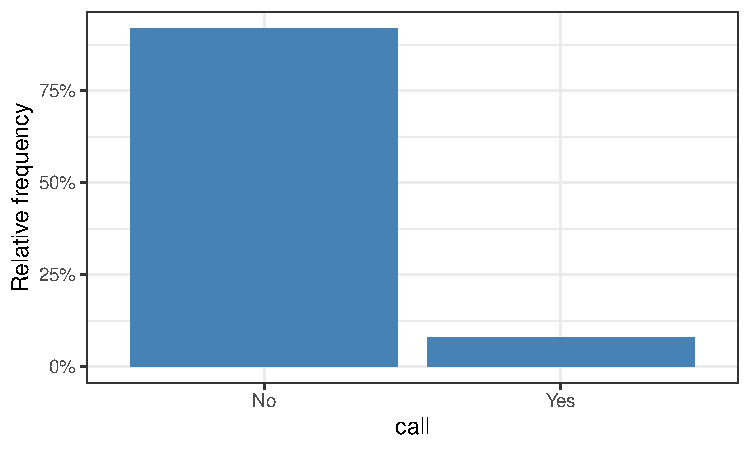
\includegraphics[width=0.45\textwidth]{graphs/l02f14b}
\end{center}

\pause

\dq{How are bar plots different than histograms?}

\pause
\colorbox{textboxgreen!75}{\parbox{0.75\textwidth}{\textit{{\tiny Bar plots are used for displaying distributions of categorical variables,  histograms are used for numerical variables. The x-axis in a histogram is a number line,  hence the order of the bars cannot be changed. In a bar plot, the categories can be listed in any order (though some orderings make more sense than others, especially for ordinal variables.)}}}}

\end{frame}

%%%%%%%%%%%%%%%%%%%%%%%%%%%%%%%%%%
\begin{frame}[fragile]{Choosing the appropriate proportion}
Does there appear to be a relationship between race and survival callback rate?
\begin{center}
\begin{tabular}{l l cc r}
					               & 			 & \multicolumn{2}{c}{{Callback}} \\
  \cline{3-4}
					               &			 & No	 & Yes	& Total \\ 
  \cline{2-5}
\multirow{2}{*}{{Race}}& Black & 2278  & 157	  	& 2435 \\ 
  					             & White & 2200	 & 235 	    & 2435 \\ 
  \cline{2-5}
  					             & Total & 4478  & 392	    &  4870 \\
  \cline{2-5}
\end{tabular}
\end{center}
\pause

To answer this question we examine the row proportions: 

\pause

\begin{itemize}

\item \% black applicants who got callback: 157 / 2435 $\approx 6.4$ \\

\pause

\item \% white applicants who got callback: 392 / 2435 $\approx 9.7$ \\

\end{itemize}

\end{frame}

%%%%%%%%%%%%%%%%%%%%%%%%%%%%%%%%%%

\begin{frame}[fragile]{Bar plots with two variables}

\begin{itemize}

\item \hl{Stacked bar plot:} Graphical display of contingency table information,
for counts.

\item \hl{Side-by-side bar plot:} Displays the same information by placing bars 
next to, instead of on top of, each other.

\item \hl{Standardized stacked bar plot}: Graphical display of contingency table 
information, for proportions.

\end{itemize}
\end{frame}

%%%%%%%%%%%%%%%%%%%%%%%%%%%%%%%%%%
\begin{frame}

\dq{What are the differences between the three visualizations shown below?}

\begin{center}
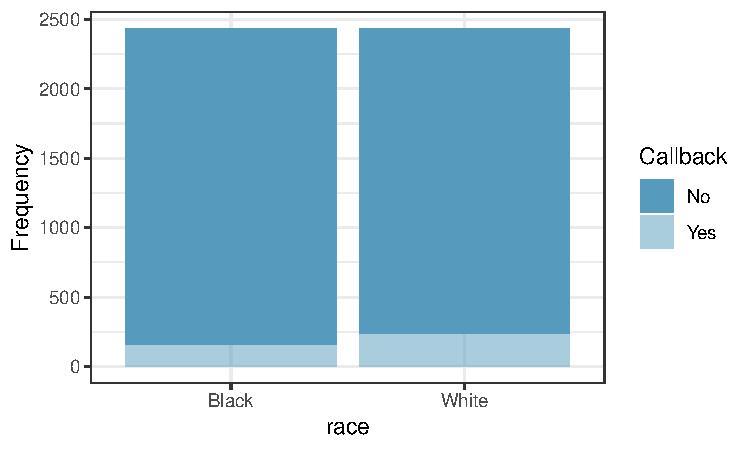
\includegraphics[width=0.45\textwidth]{graphs/l02f15a}
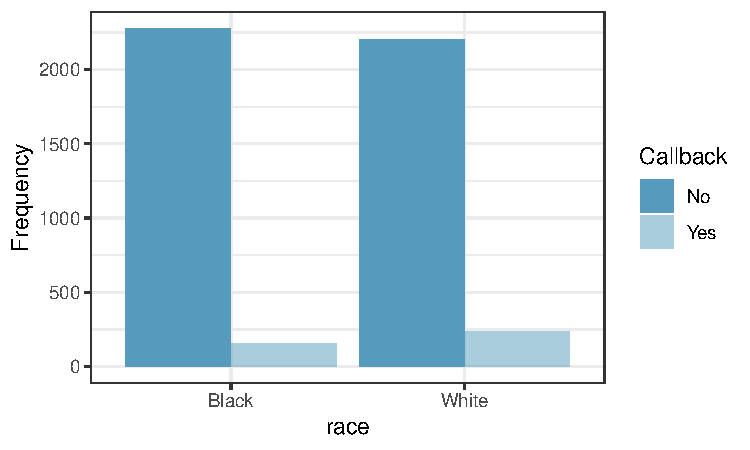
\includegraphics[width=0.45\textwidth]{graphs/l02f15b} \\
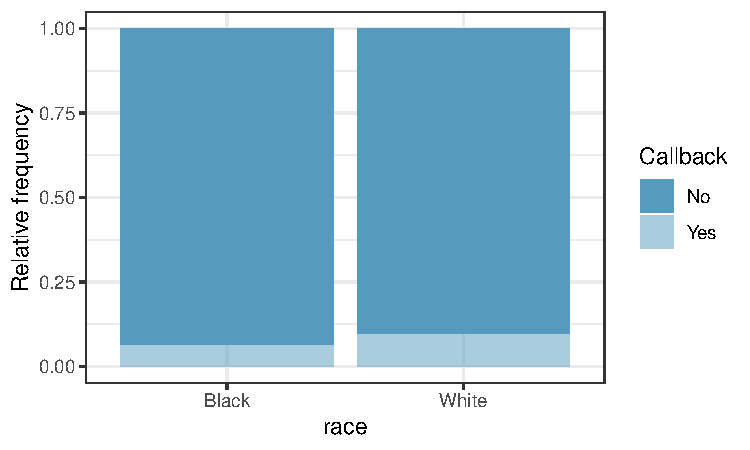
\includegraphics[width=0.45\textwidth]{graphs/l02f15c}
\end{center}

\end{frame}


%%%%%%%%%%%%%%%%%%%%%%%%%%%%%%%%%%
\begin{frame}
\frametitle{Side-by-side box plots}

\dq{Does there appear to be a relationship between type of vehicle and miles per gallon?}

\begin{center}
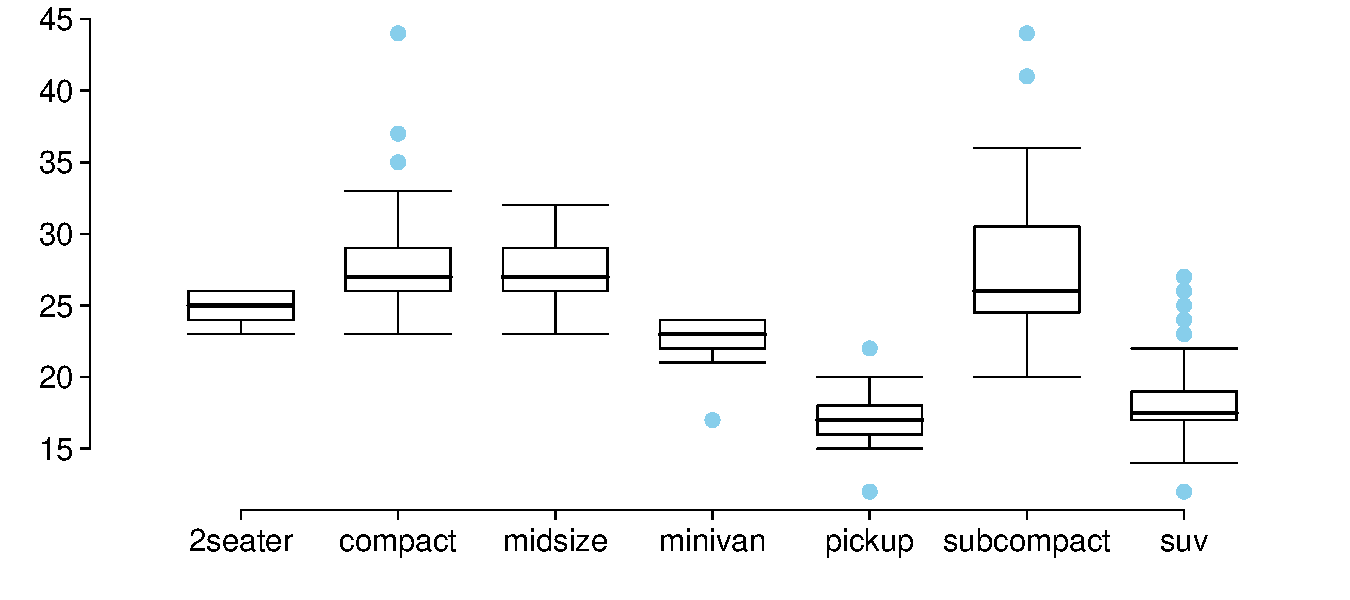
\includegraphics[width=\textwidth]{graphs/l02f16}
\end{center}
\end{frame}

%%%%%%%%%%%%%%%%%%%%%%%%%%%%%%%%%%
\section{Case Study}
%%%%%%%%%%%%%%%%%%%%%%%%%%%%%%%%%%
\begin{frame}
\frametitle{Racial discrimination}
\begin{center}
\colorbox{textboxred!85}{\parbox{0.75\textwidth}{As we saw earlier, there is difference of about 3\% in callback between CVs with white names and those with African-American names.}}
\end{center}
\end{frame}
%%%%%%%%%%%%%%%%%%%%%%%%%%%%%%%%%%
\begin{frame}{Practice}

\pq{We saw a difference of almost 3\% between the proportion of African-American and White CVs getting callbacks. Based on what we know, there are many things to consider.}

\begin{enumerate}[(a)]

\item If we were to repeat the experiment we will definitely see that more African-American names get callback. This was a fluke.

\item Callback is dependent on race, White-sounding names are more likely to get callback, and hence there is racial discrimination against African American job-seekers.

\item The difference in the proportions of callback is due to chance, this is not  evidence of racial discrimination against African-Americans in labour market. 

\item African-American are less qualified than White job-applicants, and this is why fewer African-American get callback.
\end{enumerate}
\end{frame}

%%%%%%%%%%%%%%%%%%%%%%%%%%%%%%%%%%
%%%%%%%%%%%%%%%%%%%%%%%%%%%%%%%%%%%%

\subsection{Competing claims}

%%%%%%%%%%%%%%%%%%%%%%%%%%%%%%%%%%%%%

\begin{frame}{Two competing claims}

\begin{enumerate}

\item ``There is nothing going on." \\
Callback and race are \hl{independent}, no racial discrimination, observed difference in proportions is simply due to chance. $\rightarrow$ \hl{Null hypothesis}

\pause

\item ``There is something going on." \\
Callback and race are \hl{dependent}, there is racial discrimination, observed difference in proportions is not due to chance. $\rightarrow$ \hl{Alternative hypothesis}

\end{enumerate}
\end{frame}

%%%%%%%%%%%%%%%%%%%%%%%%%%%%%%%%%%%%%%%%%
\begin{frame}
\frametitle{Recap: hypothesis testing framework}

\begin{itemize}
\item We start with a \hl{null hypothesis ($H_0$)} that represents the status quo.
\item We also have an \hl{alternative hypothesis ($H_A$)} that represents our research question, i.e. what we're testing for.
\item We conduct a hypothesis test under the assumption that the null hypothesis is true, either via simulation (today) or theoretical methods (later in the course).
\item If the test results suggest that the data do not provide convincing evidence for the alternative hypothesis, we stick with the null hypothesis. If they do, then we reject the null hypothesis in favor of the alternative.
\end{itemize}
\end{frame}
%%%%%%%%%%%%%%%%%%%%%%%%%%%%%%%%%%%%%%%%%
\subsection{Testing via simulation}

%%%%%%%%%%%%%%%%%%%%%%%%%%%%%%%%%%%%%

\begin{frame}
\frametitle{Simulating the experiment...}

... under the assumption of independence, i.e. leave things up to chance. \\

\vspace{0.5cm}

If results from the simulations based on the \hl{chance model} look like the data, then we can determine that the difference between the proportions of promoted files between White and African-American job-applicants was simply \hl{due to chance} (callback and race are independent). \\

\vspace{0.5cm}

If the results from the simulations based on the chance model do not look like the data, then we can determine that the difference between the proportions of promoted files between White and African-American job-applicants was not due to chance, but \hl{due to an actual effect of race} (callback and race are dependent).

\end{frame}

%%%%%%%%%%%%%%%%%%%%%%%%%%%%%%%%%%

\begin{frame}
\frametitle{Simulation Result}
\begin{center}
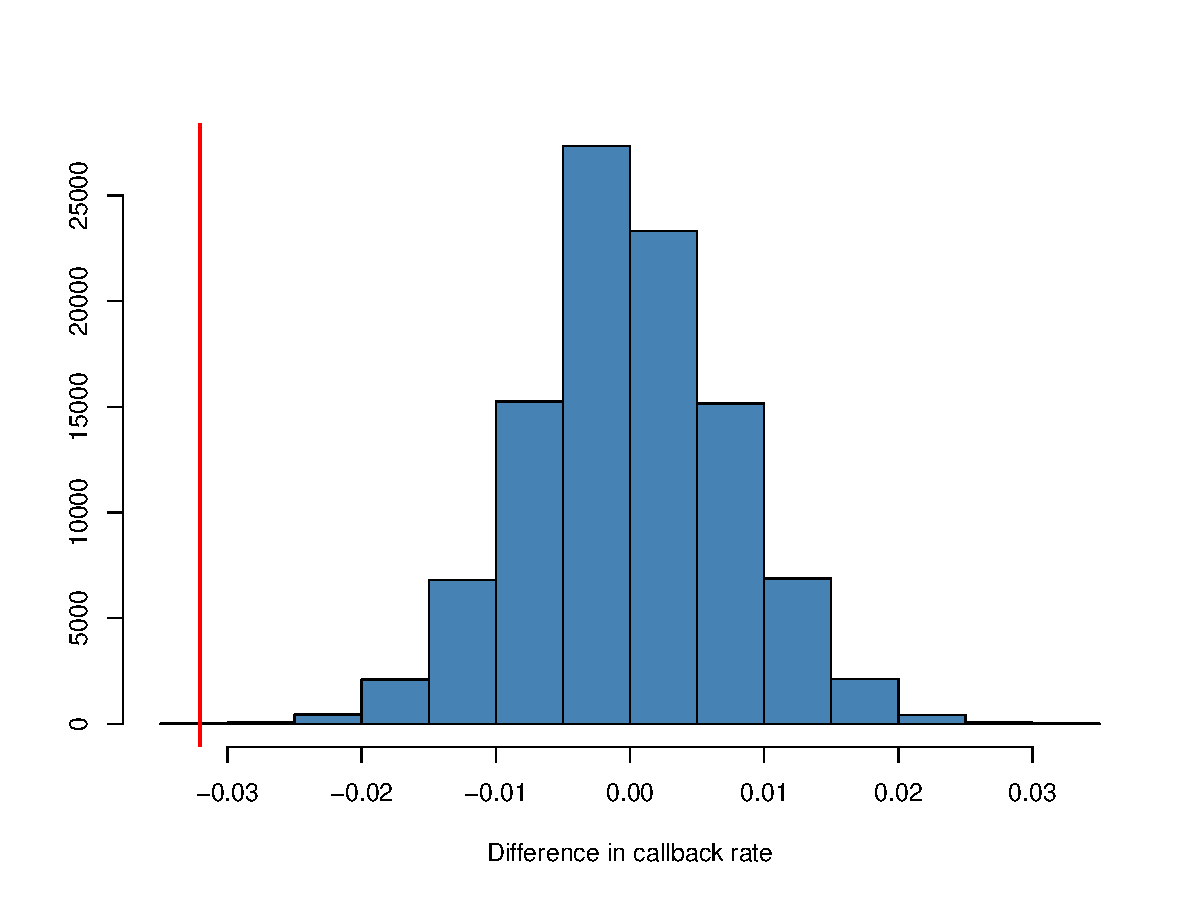
\includegraphics[width=0.7\textwidth]{graphs/l02f17}
\end{center}
\end{frame}


%%%%%%%%%%%%%%%%%%%%%%%%%%%%%%%%%%


\end{document}
